%!TEX root = main_ISMB.tex
\section{Supplementary data}
\subsection{RNAinverse}
Using the same dataset of $50$ structures, we generated $100$ samples
per structure with \RNAinverse. They yield for most parameters
a high entropy. We present for every different concentration of \texttt{C+G}
the average sample entropy and the average base pairs entropy.


\begin{figure}[ht!]
	\centering
	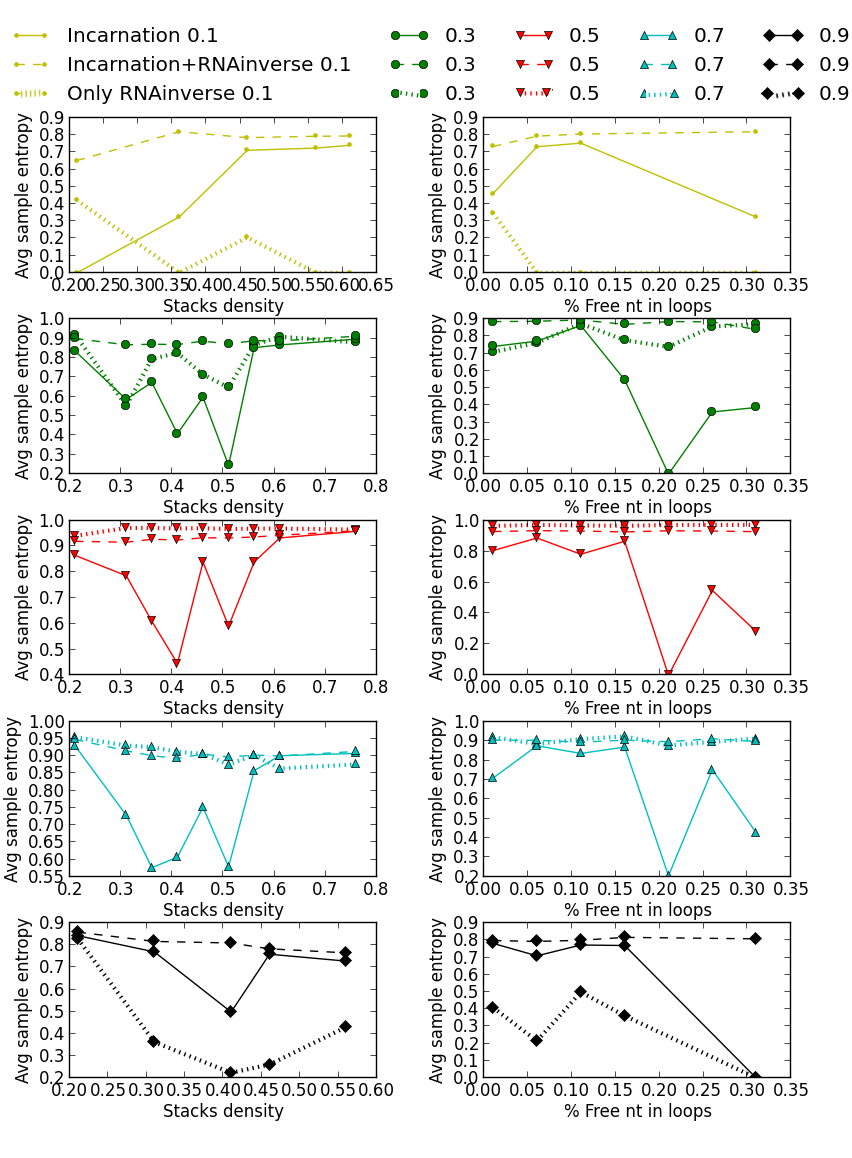
\includegraphics[scale=0.4]{Figures/RNAinverse_data_100.png}
	\caption{Entropy and \texttt{C+G} content.}
	\label{fig:rnainverse}
\end{figure}